\documentclass{article}

% Language setting
% Replace `english' with e.g. `spanish' to change the document language
\usepackage[spanish]{babel}
\usepackage[most]{tcolorbox}

% Set page size and margins
% Replace `letterpaper' with `a4paper' for UK/EU standard size
\usepackage[letterpaper,top=2cm,bottom=2cm,left=3cm,right=3cm,marginparwidth=1.75cm]{geometry}

% Useful packages
\usepackage{amsmath}
\usepackage{graphicx}
%\usepackage{subfigure}
\usepackage{caption}
\usepackage{subcaption}
\usepackage[colorlinks=true, allcolors=blue]{hyperref}
\usepackage{algorithm2e}

\newtcolorbox[auto counter, number within=section]{exercise}[1][]{
    colback=blue!5!white,
    colframe=blue!75!black,
    fonttitle=\bfseries,
    title=Ejercicio \thetcbcounter,
    #1 % Allows you to add custom options locally (like labels)
}


\title{Algoritmos de búsqueda en árboles}
\author{Arturo Gil y Juan José Cabrera}

\begin{document}
\maketitle

\section{Introducción}
En esta práctica utilizaremos y programaremos diferentes algoritmos de búsqueda en árbol. Durante las clases magistrales de la asignatura hemos planteado diferentes tipos de problemas y soluciones que se pueden relacionar con lo que veremos en esta sesión, por ejemplo:
\begin{itemize}
    \item Problemas de tipo 8-puzzle.
    \item Hallar el trayecto con menor cantidad de transbordos entre dos estaciones de metro o autobús.
    \item Búsqueda del camino más corto entre dos ciudades.
\end{itemize}

\section{El problema}
Nos centraremos en un problema de búsqueda de rutas entre dos ciudades. Trabajaremos inicialmente con el mapa mostrado en la figura \ref{fig:mapa_carreteras}. Se trata de un mapa de carreteras de España simplificado. Los ejes X e Y de la gráfica (grados) muestran la posición GPS de algunas ciudades españolas (nodos de la red). Entre los nodos de la red \textbf{se han anotado la distancia en kilómetros cuando se circula por carretera entre ellos}. Durante el resto de la práctica, abordaremos los siguientes objetivos:
\begin{itemize}
    \item Ser capaces de representar grafos de forma sencilla en python.
    \item El manejo de listas y diccionarios en python para problemas de búsqueda en árboles.
    \item La programación de los algoritmos siguientes para la búsqueda de rutas óptimas entre ciudades
    \begin{itemize}
        \item Breadth-first search BFS: búsqueda en anchura.
        \item Búsqueda greedy (ávara) y
        \item $A^*$ (el algoritmo A estrella). 
    \end{itemize}        
\end{itemize}


\begin{figure}
    \centering
    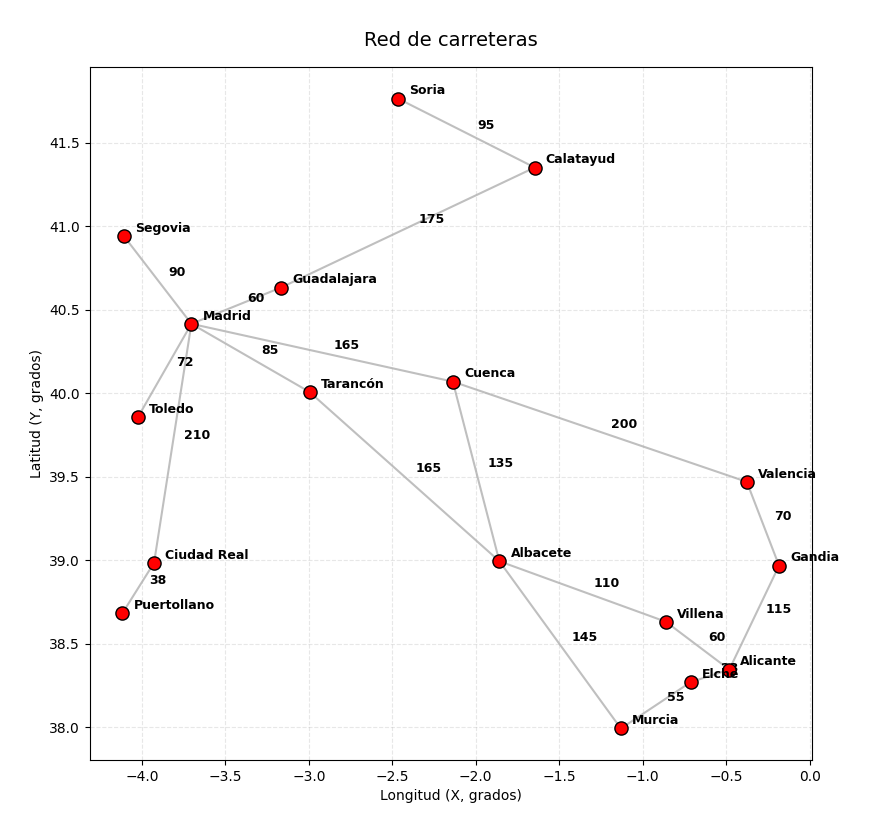
\includegraphics[width=0.9\linewidth]{figures/mapa_carreteras.png}
    \caption{Un mapa de carreteras de España simplificado. Se muestra la distancia por carretera entre los diferentes nodos y la posición GPS (grados) de cada nodo.}
    \label{fig:mapa_carreteras}
\end{figure}

\subsection{Materiales}
Utilizaremos el repo Intro2AI: \url{https://github.com/4rtur1t0/Intro2AI}. Usaremos los ficheros del directorio \texttt{practice\_search\_algorithms}. Dentro de este directorio, encontramos:
\begin{itemize}
    \item \texttt{search\_algorithms.py}: fichero principal de la práctica. Desde aquí llamaremos al resto de algoritmos que vamos a programar y a probar.
    \item \texttt{graph/graph.py}: una clase \texttt{Graph} con una implementación sencilla de un grafo no dirigido en python.
    \item \texttt{search\_algorithms}: un paquete de python donde el estudiante deberá implementar sus algoritmos de búsqueda en árboles para después poderlos probar.
\end{itemize}

\subsection{¿Cómo representar un árbol en python?}
Como ayuda, la clase \texttt{Graph} se proporciona ya programada, pues queremos que el/la estudiante se concentre en implementar los algoritmos de búsqueda sin tener que crear toda la estructura del programa desde cero. También, se han proporcionado una serie de funciones al estudiante que le facilitarán el trabajo, por ejemplo:  una función para dibujar el grafo, encontrar un nodo en el grafo, encontrar la distancia entre dos nodos o calcular la distancia en línea recta hasta un nodo.

\begin{exercise}
En este momento es importante que entienda cómo se ha programado el grafo. \\

\textbf{EJERCICIO}\\
Observe el resultado de la línea \texttt{print(spain\_network.graph)} del script \texttt{search\_algorithms.py}. Alternativamente, observe la variable \texttt{print(spain\_network.graph)} en el depurador (figura \ref{fig:grafo_dict}).    
\end{exercise}

Veamos, a continuación, algunos ejemplos en el diccionario \texttt{spain\_network.graph} (clase \texttt{Graph()}):
\begin{verbatim}
{'Madrid': {'Ciudad Real': 210, 'Cuenca': 165, 'Guadalajara': 60, 
            'Segovia': 90, 'Tarancón': 85, 'Toledo': 72},
 'Cuenca': {'Albacete': 135, 'Madrid': 165, 'Valencia': 200},
 'Albacete': {'Cuenca': 135, 'Murcia': 145, 'Tarancón': 165, 'Villena': 110}, ...}
\end{verbatim}

Este diccionario está indicando que Madrid está conectado con Ciudad Real, Cuenca, Guadalajara, Segovia, Tarancón y Toledo. Cada uno de los valores en el diccionario guarda la distancia (en kilómetros) por carretera. A su vez Cuenca está conectada con Albacete, Madrid y Valencia. Para encontrar todos los nodos que están conectados con Cuenca, hacemos (accedemos a la clave \texttt{'Cuenca'}):
\begin{verbatim}
    print(spain\_network.graph['Cuenca'])    
\end{verbatim}

\textbf{Nos debemos fijar que la variable \texttt{spain\_network.graph} es un diccionario de diccionarios} (pues en cada par \textit{key-value}, \textit{value} es un diccionario también). Para ver la distancia entre Cuenca y Valencia, accedemos a:
\begin{verbatim}
    print(spain\_network.graph['Cuenca']['Valencia']) 
\end{verbatim}

Obviamente, debemos obtener el mismo resultado si buscamos la distancia entre Valencia y Cuenca:
\begin{verbatim}
    print(spain\_network.graph['Valencia']['Cuenca']) 
\end{verbatim}

Esta no es la forma más eficiente de guardar un grafo, pero sí la más legible y fácil de entender (por esta razón se ha elegido esta representación en la práctica). La clase \texttt{Graph()} cuenta con varios métodos que nos permiten manejar el grafo con facilidad:
\begin{verbatim}
    def get_node(self, name):        
    def get_distance(self, node1, node2):
    def get_neighbors(self, node):    
    def compute_flying_distance(self, node1, node2):
\end{verbatim}

% \begin{itemize}
%     \item \texttt{def get\_node(self, name)}: devuelve un nodo del grafo.
%     \item \texttt{def get\_distance(self, node1, node2)}: devuelve la distancia por carretera entre dos nodos del grafo.
%     \item \texttt{def get\_neighbors(self, node)}: devuelve los nodos que están conectados con el especificado.
% \end{itemize}
   

\begin{exercise}
Con esto, abra el fichero \texttt{search\_algorithms.py}. Verá las siguientes líneas de ćodigo:
\begin{verbatim}
    if __name__ == "__main__":
        spain_network = Graph()
        spain_network.build_network()
        print(spain_network.graph)
        spain_network.plot_network()
\end{verbatim}
% Ejecute el fichero y observe el grafo.\\
\textbf{EJERCICIO}\\
Utilice las siguientes funciones sobre el objeto \texttt{spain\_network} y anote el resultado: ¿qué hace cada función? ¿Qué resultado se obtiene?
\begin{verbatim}
    get_node(self, name)
    get_distance(self, node1, node2)
    def get_neighbors(self, name)
    def compute_flying_distance(self, ciudad1, ciudad2)
\end{verbatim}
Puede consultar la implementación de cada función en la clase \texttt{graph/Graph()}.
\end{exercise}



\subsection{Búsqueda en anchura (\textit{breadth-first search})}
Un algoritmo de búsqueda en anchura o Breadh-first Search (BFS) explora el árbol según el pseudo-código mostrado en el  Algoritmo \ref{alg:bfs}. El algoritmo explora en un orden fijo todos los nodos de la red hasta encontrar una solución. Los nodos se exploran por niveles utilizando una cola FIFO (\textit{First In}, \textit{First Out}). Los niveles se definen en base a los saltos que hay que dar para conectar el nodo inicial (\textit{root}) con cualquier otro nodo. 
La característica principal del algoritmo BFS consiste en que se asegura la exploración de todos los nodos de un nivel antes de pasar al siguiente nivel. Este forma de explorar el árbol se muestra en la figura \ref{fig:bfs}, donde se describe también el contenido de la cola abierta FIFO (\textit{open queue}) que se emplea para almacenar los nodos que se pretenden visitar.

Para nosotros, la cola abierta será simplemente una lista de python con los nombres de los nodos, donde añadiremos elementos por la derecha (\texttt{append}) y los eliminaremos por la izquierda (\texttt{pop(0)}). Un ejemplo de cómo se procesa el árbol lo vemos en la figura \ref{fig:cola_bfs}. El funcionamiento del algoritmo \ref{alg:bfs} lo podemos describir de la manera siguiente:
\begin{itemize}    
    \item Se inicializa la cola abierta del algoritmo (cola FIFO, \textit{open queue}) con el nodo inicial (este es el nodo inicial desde el que queremos encontrar el camino).
    \item Se inicializa la lista cerrada (\texttt{self.closed\_queue}). Inicialmente, esta lista estará vacía. Después, contendrá los nodos que ya han sido explorados.
    \item Se inicializa un diccionario (\texttt{node\_info}) que contiene información sobre el padre de cada nodo (\textit{id est}, desde qué nodo se ha llegado a cada nodo). El nodo inicial se marca con \texttt{None}, pues no tiene padre.
    \item El algoritmo prosigue, indicando que mientras haya elementos dentro de la cola abierta:
    \begin{itemize}
        \item Se extrae un elemento por la izquierda de la cola abierta (\texttt{queue.pop()}).
        \item Si el nodo actual es igual al nodo buscado (\texttt{destination\_node}), se termina la búsqueda y se calcula la ruta.
        \item En caso contrario, se procesa el nodo actual. El procesado del nodo actual se debe hacer en la función (\texttt{process\_neighbours}). Dentro de esta función:
        \begin{itemize}
            \item Se buscan los nodos vecinos que están conectados al nodo actual (\texttt{neighbours}). Para cada nodo vecino:
            \begin{itemize}
                \item Si el nodo está en la lista cerrada: \texttt{continue}, pues ya ha sido explorado anteriormente.
                \item Así pues, si el nodo vecino no está en la lista cerrada, se añadirá a la lista abierta (si no existe en la lista abierta). En este mismo momento, se añadirá el nodo vecino y su padre en el diccionario \texttt{self.parent\_info}
            \end{itemize}
        \end{itemize}
    \end{itemize}
\end{itemize}


\begin{figure}  
    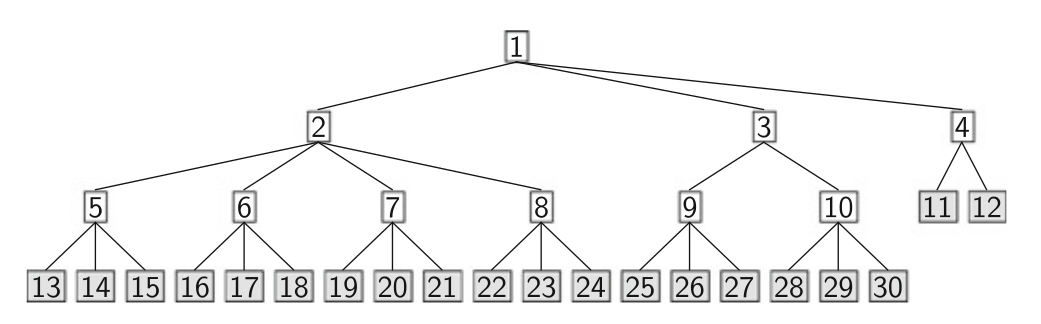
\includegraphics[width=0.8\linewidth]{figures/bfs.png}
    \caption{Un árbol y el orden en el que se exploran los nodos en \textit{breadth-first search}.}
    \label{fig:bfs}
\end{figure}

\begin{figure}
    \centering
    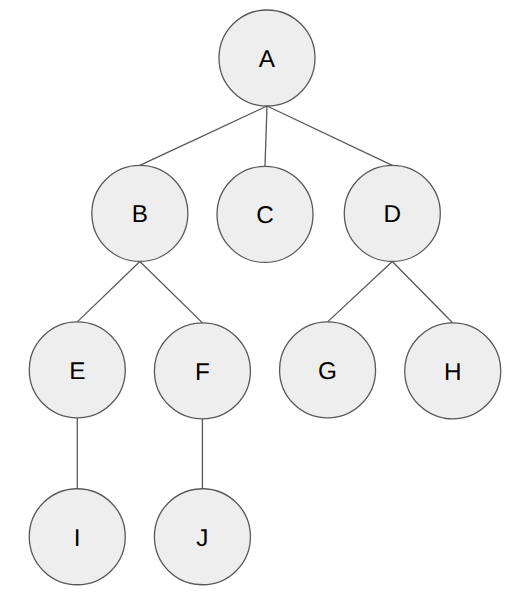
\includegraphics[width=0.3\linewidth]{figures/nodos_bfs.png}
    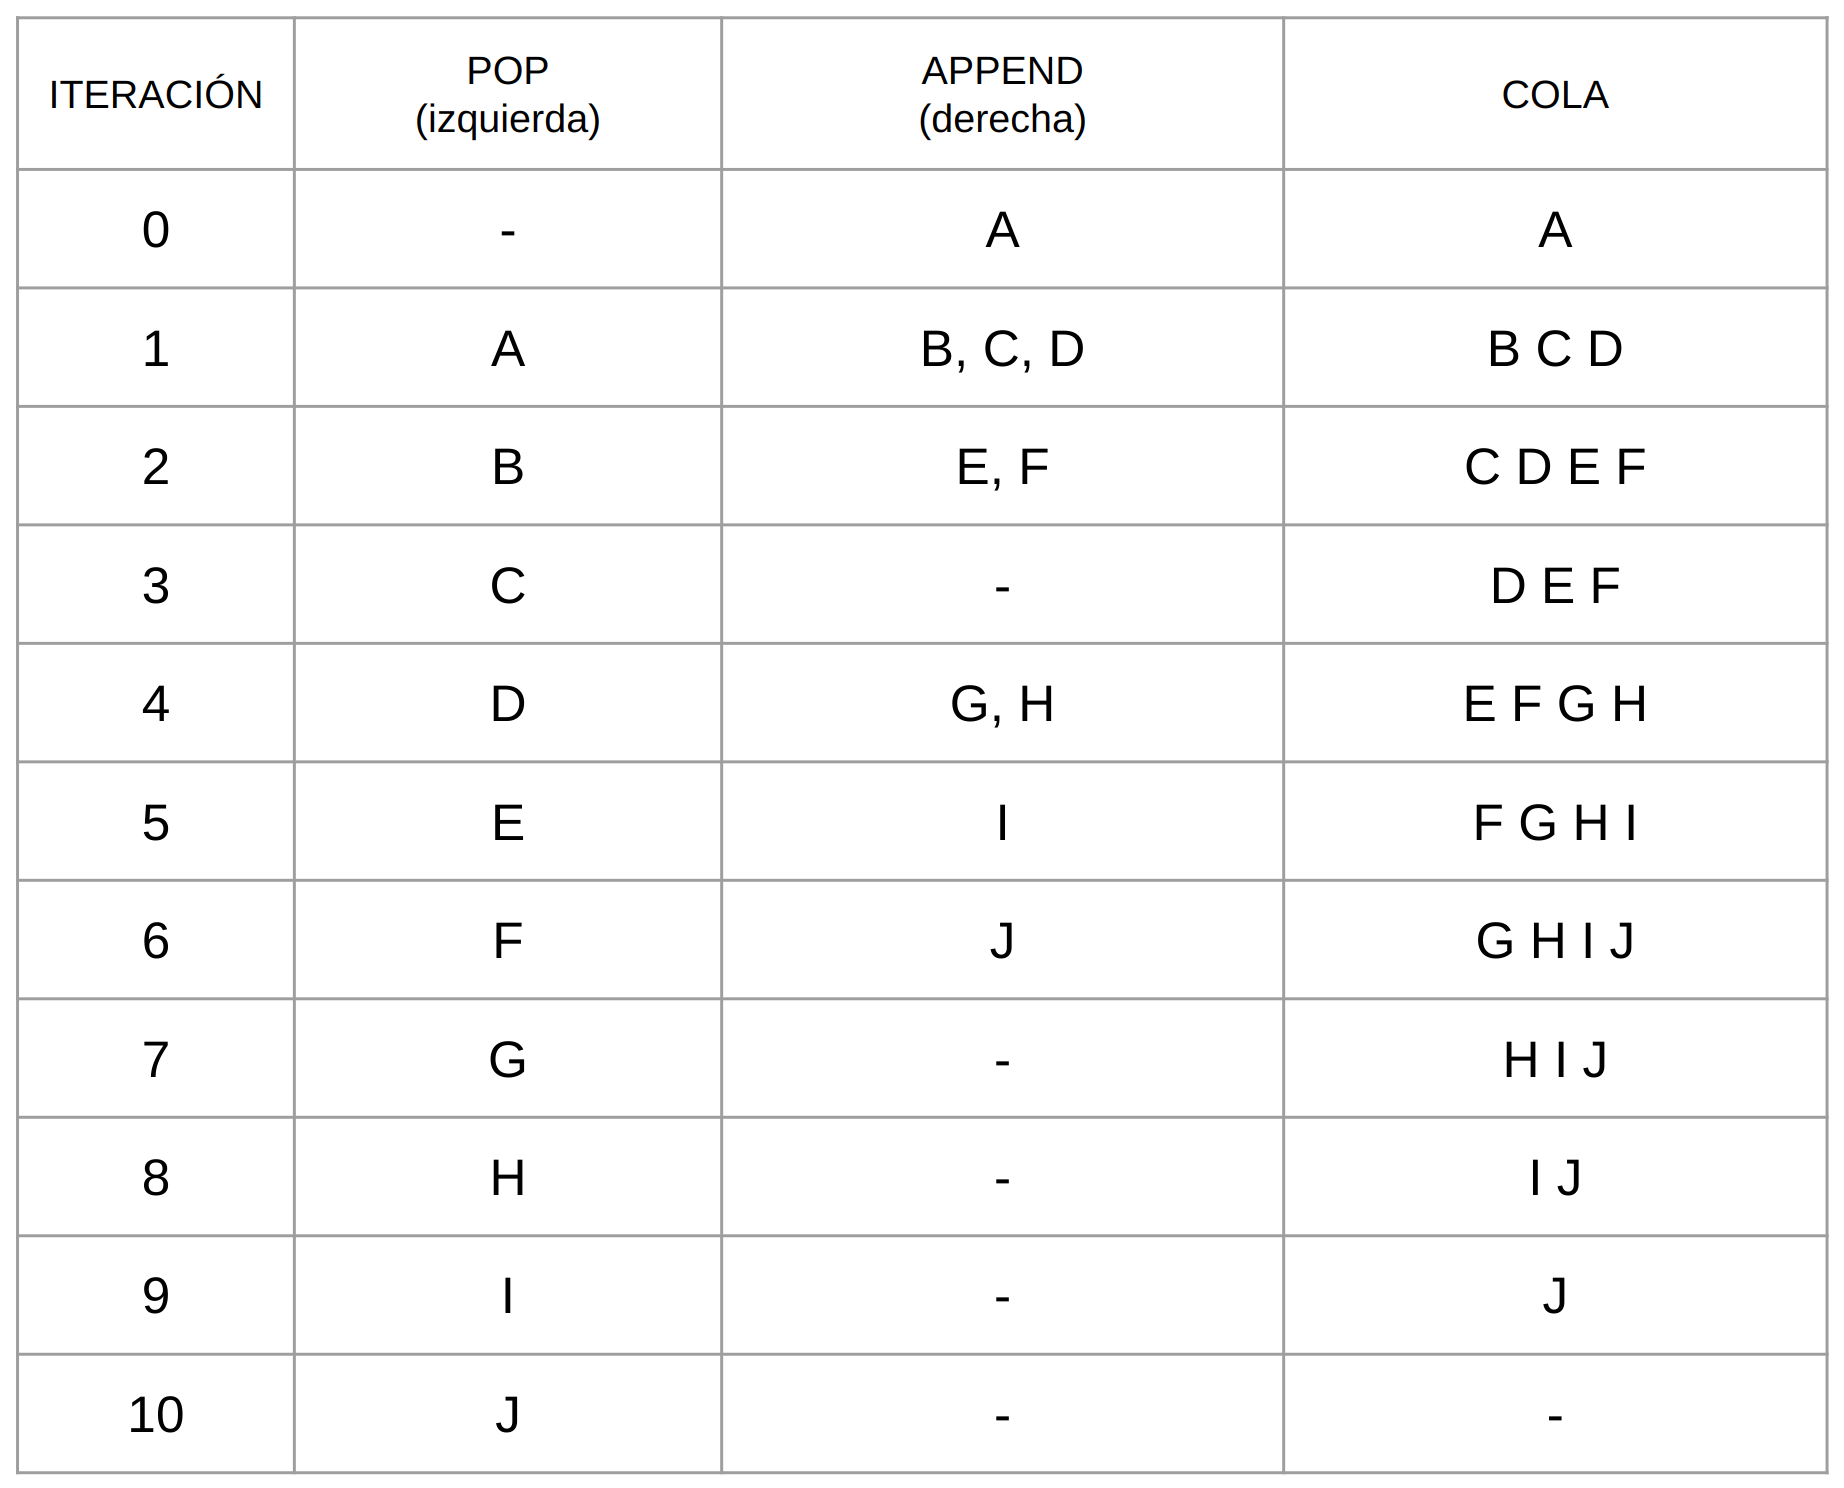
\includegraphics[width=0.5\linewidth]{figures/cola_bfs.png} 
    \caption{Izquierda: un árbol. Derecha: el orden en el que se exploran los nodos, las operaciones de \textit{pop} y \textit{append}y la cola del algoritmo \textit{breadth-first search} en cada una de sus iteraciones.}
    \label{fig:cola_bfs}
\end{figure}

\begin{figure}
    \centering
    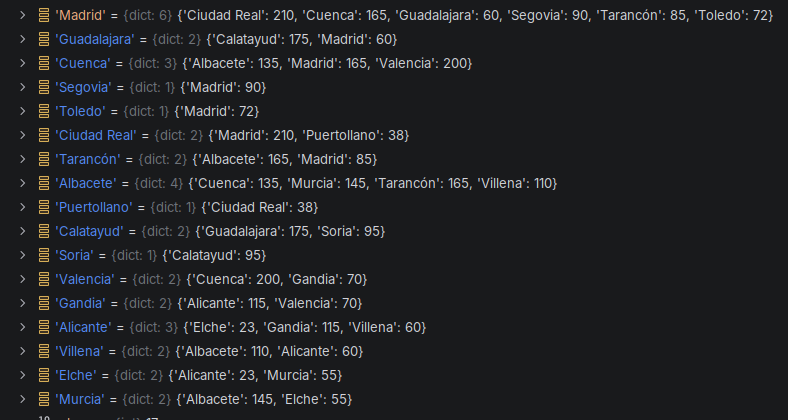
\includegraphics[width=0.8\linewidth]{figures/grafo_dict.png}
    \caption{Un diccionario en python representando un grafo.}
    \label{fig:grafo_dict}
\end{figure}

\SetKwComment{Comment}{/* }{ */}

\begin{algorithm}
\caption{El algoritmo BFS.}\label{alg:bfs}
\KwData{\\
start = root\_node\\end = end\_node\\
open\_queue = [root\_node]\\
closed\_queue = []\\
node\_info = \{root\_node: None\}}
\KwResult{result = [$node_x, node_y, node_z, \ldots$]}
\While{len(queue)$>0$}{
    node = open\_queue.pop(0)\\
    closed\_queue.append(node)\\
  \eIf{node == end\_node}{
    route = compute\_route(node\_info);\\
    return route;
  }{
    /* Se añaden los vecinos del nodo actual a la cola*/\\   
    process\_neighbors(node)
  }
}
\end{algorithm}

\begin{algorithm}
\caption{Process neighbours.}
\label{alg:process_neighbours}
\KwData{current\_node}
\KwResult{None}
neighbours = get\_neighbours(current\_node)\\
\For{(neighbour in neighbours)}{
    \If{neighbour in closed\_queue}
        {continue}
    \If{neigbour not in visited\_nodes}{
        add neighbour to the open queue\\
        store parent information
        }
    }
\end{algorithm}
   


\begin{exercise}
Continuamos la práctica y seguimos leyendo el fichero \texttt{search/search\_algorithms.py}. Descomente las siguientes líneas de ćodigo:
\begin{verbatim}
    algoritmo = BFS_Algorithm(spain_network)
    origen = 'Madrid'
    destino = 'Elx'
    route, distance, iterations = algoritmo.find_route(origen, destino)
\end{verbatim}


\textbf{EJERCICIO}\\
\begin{itemize}
    \item Encuentre la clase \texttt{BFS\_Algorithm}. Esta clase la encontrarás en el fichero de python \texttt{search\_algorithms/bfs\_algorithm.py}. La clase implementa el algoritmo BFS que se ha explicado.
    \item Encuentre la función \texttt{find\_route} deberá entender las líneas del algoritmo y relacionarlas con el algoritmo BFS que ya se ha expuesto.
\end{itemize}
\end{exercise}

\begin{exercise}
Deseamos entender cómo evoluciona la cola abierta (\texttt{self.open\_queue}) y la cola cerrada \texttt{self.closed\_queue} del algoritmo en cada iteración. También es interesante comprender cómo funciona la variable \texttt{self.node\_info} (información de los nodos) y la lista de vecinos en la función \texttt{process\_neighbors}.\\

\textbf{EJERCICIO}\\
\begin{itemize}
    \item[a)] Modifique la función \texttt{find\_route} para que imprima por pantalla estas 4 variables. Se recomienta que escriba una función \texttt{print\_info} que se encargue de imprimir esta información.
    \item[b)] Ejecute la función \texttt{find\_route} paso por paso usando el modo debug. Anote en papel una tabla como la mostrada en la figura \ref{fig:cola_bfs}. Anote el contenido de la lista cerrada y abierta en las 3 primeras iteraciones.
    \item[c)] Siga el progreso de las listas abierta, cerrada y los vecinos en el mapa de la figura \ref{fig:mapa_carreteras}.
\end{itemize}    
\end{exercise}

Es fácil ver cómo se van añadiendo los nodos a la cola abierta (\texttt{self.open\_queue}) y cerrada (\texttt{self.closed\_queue}). Nos tenemos que dar cuenta de que los nodos en la cola se procesan por la izquierda. Los nuevos nodos que se encuentran conectados al nodo actual se añaden por la derecha. Con esta acción, nos aseguramos de que todos los nodos conectados a un nivel determinado hayan sido procesados antes de avanzar hacia un nivel más bajo. En la práctica nos debemos dar cuenta de que el algoritmo busca ``en anillos'' expandiéndose desde el nodo inicial hasta dar con el nodo final.


\subsubsection{Detalles importantes}
Hay un detalle importante que hemos soslayado: el mapa mostrado es un tipo especial de árbol en el que un nodo hijo puede estar conectado con varios padres (podemos llegar a Albacete desde Cuenca o Tarancón). Para guardar la ruta final en un algoritmo BFS en el caso en el que un nodo pueda ser visitado desde diferentes padres, la mejor estrategia es utilizar un diccionario de padres (\texttt{node\_info}): como el algoritmo BFS explora el grafo por niveles (saltos), la primera vez que se visita cualquier nodo se tiene la garantía de que se ha llegado a él con el mínimo número de saltos. Así pues, si, posteriormente, se llega al mismo nodo por otro camino (desde otro padre), el número de saltos será igual o mayor que en el primer caso. En consecuencia, solamente se debe añadir el nodo a la cola la primera vez que se vea. Esto se puede observar en el algoritmo BFS que se ha programado, pues solamente se añade un nodo al diccionario \texttt{node\_info} si no está en \texttt{closed\_queue} y tampoco está en \texttt{open\_queue}.

\begin{exercise}
Es importante ver cómo se reconstruye el camino que constituye la solución. Cuando, finalmente, el nodo actual coincide con el nodo de destino, se llama a la función \texttt{reconstruct\_route}.\\

\textbf{EJERCICIO}\\ 
Programe la función \texttt{reconstruct\_route}. La función debe consultar el diccionario \texttt{parent\_info} y construir la ruta desde el final hasta el principio. Como ayuda, imprima por pantalla el nodo actual y su padre mientras se construye la ruta. Calcule la distancia total de la ruta para que sea devuelta por el algoritmo.
\end{exercise}


\subsubsection{Pruebas finales}
Para finalizar, haremos una serie de pruebas para poder observar las características más importantes del algoritmo. En un algoritmo de búsqueda en grafos, nos interesa saber, principalmente:
\begin{itemize}
    \item ¿Cuántas iteraciones son necesarias para encontrar una solución entre dos nodos del grafo?
    \item ¿Cuántos nodos se han tenido que expandir para encontrar una solución?
\end{itemize}

Ambos factores determinan el tiempo de cómputo del algoritmo. El segundo factor está relacionado con la cantidad de memoria que necesita el algoritmo para encontrar una solución. En este ejemplo tenemos muy pocos nodos: el tiempo de cómputo y la necesidad de memoria son factores importantes en problemas búsqueda reales, como el que veremos al final de esta práctica.

\begin{exercise}
Se desea calcular el número de iteraciones realizadas y el tamaño máximo de las colas (abierta y cerrada). Esto nos dará una idea del consumo en tiempo y memoria del algoritmo.\\

\textbf{EJERCICIO}\\ 
Modifique el código de la función \texttt{find\_route} para contar el número de iteraciones del algoritmo y el número de nodos que se han añadido a la cola.
\end{exercise}

\begin{exercise}
Necesitamos tener una batería de pruebas de nuestro algoritmo. Probaremos con un conjunto de nodos de origen y destino.\\

\textbf{EJERCICIO}\\
Modifique los puntos de origen y destino en el fichero \texttt{search\_algorithms.py}. Después de 10 pruebas diferentes, 
\begin{itemize}
    \item Compruebe si en todos los casos se encuentra una solución.
    \item Anote la ruta obtenida, la distancia, el número de iteraciones del algoritmo y el número de nodos expandidos.
    \item Suponga que se ha encontrado una ruta entre dos ciudades del mapa. ¿La distancia total por carretera entre las dos ciudades es mínima? 
    \item ¿El número de saltos entre nodos consecutivos de la ruta entre las ciudades es mínimo?
\end{itemize}      
\end{exercise}

Después de haber jugado un poco con el algoritmo y haber buscado rutas entre diferentes nodos del mapa, nos debemos dar cuenta de que:
\begin{itemize}
    \item Si existe una ruta entre dos nodos del mapa, la ruta encontrada por BFS es aquella con el menor número de saltos entre nodos.
    \item De ninguna manera, la ruta hallada es mínima en términos de distancia: es mínima en términos del número de saltos entre nodos.
\end{itemize}

Por ejemplo, si buscamos una ruta entre Madrid y Elx, obtendremos:
\begin{verbatim}
Found destination! In iterations:  17
Route found: Madrid -> Cuenca -> Albacete -> Murcia -> Elx
TOTAL DISTANCE IS:  500
    \end{verbatim}
Así pues, el algoritmo necesita 17 iteraciones para encontrar una ruta entre las dos ciudades. La ruta obtenida tiene un número de saltos mínimo (4, 4 flechas). La distancia obtenida (500 km) no es la mínima entre los nodos (pues el algoritmo no usa ninguna información de distancia).

\subsubsection{Aplicaciones}
Podríamos preguntarnos para qué aplicaciones nos interesaría saber la distancia entre dos nodos en base al número de saltos. Se anotan algunas situaciones:
\begin{itemize}
    \item \textbf{Protocolos de enrutamiento de red}: en el algoritmo RIP (\textit{Routing Information Protocol}), los routers utilizan la cuenta de saltos (\textit{hop count}) para encontrar el camino que necesita el menor número de \textit{routers} intermedios para enviar los datos entre dos puntos de internet. Esta es una cuestión importante, pues en un \textit{router} se produce siempre un retardo en el mensaje (al tener que procesar el mensaje y enrutarlo a otra red). La distancia total entre el nodo inicial y el final es menos relevante que el número de nodos intermedios: piense que entre dos nodos la transmisión de información se puede hacer usando fibra óptica y donde los datos viajan a la velocidad de la luz (en ese medio).
\item \textbf{Algoritmos para la transmisión de datos en redes radio de tipo \textit{mesh}}: en las redes de radio de tipo \textit{mesh} (por ejemplo, cuando se usan sistemas de radio XBee), cada elemento de la red está conectado con otros elementos de tipo radio. En este tipo de redes se precisa que haya el menor de saltos entre el emisor y el receptor del mensaje, mientras que se limita el número de veces que hay que retransmitir el mensaje.
\end{itemize}












\subsection{\textit{Greedy search}}
El algoritmo BFS que hemos visto se clasifica como un algoritmo de búsqueda no informado, pues no dispone de ninguna información que le indique si se está acercando al nodo que se está buscando o si se encuentra cerca de encontrar una ruta válida hasta él.

Seguidamente, vamos a partir del algoritmo BFS y lo vamos a modificar utilizando una información de distancia. En concreto, vamos a utilizar un función heurística $h(s)$ que llamaremos ``distancia en línea recta'' o ``\textit{flying distance}''. En vez de expandir los nodos de la cola en un orden fijo, vamos a expandir primero el nodo de la cola que tenga un valor de $h(s)$ menor. Esta forma de proceder se denomina, generalmente, avara (Greedy), de ahí que este algoritmo se denomine \textit{Greedy Best-First Search}.

En este algoritmo avaro (\textit{greedy}), se calcula la función $h(s)$ para cada nodo de la cola abierta (\texttt{self.open\_queue}) y, a continuación, se reordena la cola en base a esta distancia. Con esto, los nodos con distancia $h(s)$ menor se quedarán a la izquierda de la cola y serán procesados antes. Con esto, en resumen, nos damos cuenta de que:
\begin{itemize}
    \item \textbf{El algoritmo BFS es de tipo no informado}, pues no usa información sobre la distancia entre los nodos o la distancia de un nodo al destino.
    \item \textbf{El algoritmo Greedy es de tipo informado} y trata de centrarse en los nodos para los que la distancia en línea recta es menor. 
\end{itemize}

En afegir una mètrica greedy basada en la distància en línia recta (flying distance) cap al destí, l'algoritme passa de ser un BFS pur a convertir-se en un Greedy Best-First Search. La cua FIFO tradicional es reemplaça per una cua que prioritza els nodes més propers al destí final. Les dues característiques principals que s'hi troben són:
\begin{itemize}
    \item \textbf{Rapidesa d'exploració}: l'algoritme ``avança'' directament en la direcció geogràfica del destí, reduint dràsticament el nombre de nodes explorats en comparació amb l'exploració en anells del BFS.

    \item \textbf{Pèrdua de la garantia d'optimitat}: a diferència del BFS estàndard, el Greedy Best-First Search no garanteix trobar el camí amb el mínim nombre de salts si hi ha obstacles, tancament de carreteres o connexions indirectes.
\end{itemize}

La clase \texttt{Graph()} proporciona una función para calcular esta distancia en línea recta. La distancia (en kilómetros) se calcula en base a la posición GPS de cada ciudad (que convenientemente se ha almacenado en un array). Para el cálculo de esta distancia se utiliza la función ``haversine'' o semiverseno que devuelve la distancia más corta entre dos puntos de una esfera:
\begin{verbatim}    
self.graph.compute_flying_distance(node_name, destination_name)
\end{verbatim}


\begin{exercise}
Se propone al estudiante que programe el algoritmo Greedy BFS partiendo del algoritmo BFS.\\

\textbf{EJERCICIO}\\
    Debe implementar el algoritmo avaro (\textit{greedy}). Para ello:
    \begin{itemize}
        \item Parta del fichero \texttt{search\_algorithms/greedy\_algorithm.py} y modifíquelo. 
        \item Modifique la función \texttt{find\_route} y \texttt{process\_neighbours}. Instrucciones: 
        \begin{itemize}
            \item En la función \texttt{process\_neighbors}, al añadir un nodo a la cola abierta, se deberá calcular la distancia en línea recta hasta el nodo destino (\textit{flying distance}). 
            \item Guarde esta información en el diccionario \texttt{self.h}.
            \item Reordene la cola abierta en base a las distancias de cada nodo al destino.
        \end{itemize}
    \end{itemize}  
    Con todo lo anterior, descomente las siguientes líneas (y comente las líneas anteriores):
    \begin{verbatim}
        algoritmo = Greedy_Algorithm(spain_network)
        origen = 'Madrid'
        destino = 'Elx'
        route, distance, iterations = algoritmo.find_route(origen , destino)
    \end{verbatim}
\end{exercise}

\begin{exercise}
    Deseamos realizar varias pruebas con el nuevo algoritmo avaro que acabamos de programar.\\
    
    \textbf{EJERCICIO}\\
    Pruebe a calcular la ruta entre Madrid y Elx. 
    A continuación, pruebe a calcular la ruta entre Elx y Madrid. ¿Se obtiene el la misma ruta (a la inversa)?¿Se obtiene la misma distancia total? ¿Considera que la ruta calculada es óptima?
\end{exercise}


\begin{exercise}
    Deseamos realizar varias pruebas con el nuevo algoritmo avaro que acabamos de programar.\\
    
    \textbf{EJERCICIO}\\
    Pruebe en total 5 rutas (p. ej. Madrid-Elx, Puertollano-Murcia, Gandía-Segovia. Para cada ruta, prueba BFS y pruebe el algoritmo Avaro:
    \begin{itemize}
        \item Anote la ruta calculada.
        \item Anote el número de iteraciones del algoritmo.
        \item Anote el número de nodos expandidos por el  algoritmo.
        \item Anote la distancia total de la ruta calculada. ¿La ruta hallada es óptima?
    \end{itemize}     
\end{exercise}

Nos debemos dar cuenta de que este algoritmo \textit{greedy} es más eficiente que el anterior en términos de iteraciones, pues siempre intenta expandir el nodo con menor distancia en línea recta. De esta manera, se dirige la búsqueda de forma más rápida hacia el destino deseado. También, el número total de nodos que se expanden es menor (si lo comparamos con BFS). Vemos, sin embargo, que la ruta que encontramos en el caso de Madrid-Elche no es óptima.

\begin{exercise}
Deseamos saber en qué punto se equivoca el algoritmo \textit{Greedy} y por qué razón.\\

\textbf{EJERCICIO}\\
Calcule a mano la ruta óptima entre Madrid y Elx: es fácil, no hay muchas combinaciones posibles. Después:
\begin{itemize}
    \item Pruebe de nuevo a hallar una ruta entre Madrid y Elx usando el algoritmo avaro.
    \item Ejecute el algoritmo paso a paso, observando los nodos y sus \textit{flying distances}.
    \item ¿En qué momento se equivoca el algoritmo avaro? ¿Por qué la ruta que se calcula no es óptima?
\end{itemize} 
\end{exercise}

Si buscamos la ruta Madrid-Elx con el algoritmo Greedy, obtenemos:
\begin{verbatim}
Found destination! in iterations: 6
Route found: Madrid -> Cuenca -> Albacete -> Villena -> Alicante -> Elche
TOTAL DISTANCE IS: 493
\end{verbatim}

Vemos que el algoritmo necesita 6 iteraciones para encontrar una ruta entre las dos ciudades. Sin duda,
utilizar $h(s)$ como heurístico permite centrar la búsqueda en los
nodos más prometedores (que están más cerca del nodo de destino, en línea recta). La ruta entre nodos tiene 5 saltos
(5 flechas), 1 más que el algoritmo BFS. La ruta obtenida entre las dos ciudades no es la que tiene una distancia mínima. En concreto, en la primera iteración, el algoritmo decide, de forma equivocada, viajar a Cuenca en vez de viajar a Tarancón. Esta decisión la toma porque Cuenca tiene una \textit{flying distance} (hasta Elche) menor que Tarancón. A partir de esa equivocación el algoritmo sigue avanzando de forma ávida hacia el destino y, además, no es capaz de enmendar su error.

\subsubsection{Detalles de implementación}
En esta práctica hemos mantenido una lista ordenada con las distancias en línea recta de cada nodo de la cola hasta el nodo final. Para ello hemos utilizado la función \texttt{sort} de python o bien \texttt{np.argsort} (de numpy). Una lista ordenada no es la estructura de datos más eficiente para esta tarea, pues realmente no necesitamos contar con los datos ordenados, sino extraer rápidamente el nodo con la mínima distancia en cada iteración. En concreto, ocurre que:
\begin{itemize}
    \item En una lista ordenada, el coste computacional de extraer el elemento mínimo (o máximo) es de tipo $O(1)$.
    \item En una lista ordenada, el coste de introducir un nuevo elemento (en su posición ordenada, claro está) es $O(N)$. Esto es fácil de entender, pues es necesario recorrer todo el array y colocar el nuevo elemento entre los índices $i-1$ e $i+1$.
    \item El coste de ordenar una lista es de tipo $O(N \log N)$.    
\end{itemize}

Si el número de nodos de la búsqueda es muy alto, es preferible utilizar una estructura de tipo Min-Heap. En concreto: 
\begin{itemize}
    \item En una Min-Heap, el coste computacional de extraer el elemento mínimo es de tipo $O(logN)$.
    \item En una Min-Heap ordenada, el coste de introducir un nuevo elemento es $O(logN)$.    
\end{itemize}

El ejemplo siguiente describe cómo definir y utilizar un Min-Heap en python.
\begin{verbatim}
import heapq
heap = []

heapq.heappush(heap, (12.5, "Node_A"))
heapq.heappush(heap, (4.2, "Node_B"))
heapq.heappush(heap, (8.9, "Node_C"))

# Consulta del mínim sense extreure'l -> O(1)
min_dist, node = heap[0]  # (4.2, 'Node_B')

# Extracció de l'element mínim: heappop() -> O(log N)
min_dist, node = heapq.heappop(heap)  # Extreu i retorna (4.2, 'Node_B')    
\end{verbatim}
    
Nota: \textbf{no es necesario hacer nada especial en este apartado}. Solamente se os proporciona esta información para que seáis conscientes de que el tiempo de cálculo es importante en cualquier algoritmo de búsqueda. Durante el resto de esta práctica  \textbf{vamos a mantener una lista ordenada, pues es más sencillo de implementar y permite al estudiante entender mejor el progreso del algoritmo.}


\subsection{A*}
El algoritmo $A^*$ es muy utilizado para el cálculo de rutas, pues comparado con el algoritmo Greedy anterior, con un poco más de esfuerzo es capaz de obtener rutas óptimas entre cualquier par de nodos de la red. Podemos pensar que el algoritmo $A^*$ es similar al algoritmo de Dijkstra: simplemente se mofifica la función de coste añadiendo una parte heurística que aproxima el coste total hasta el final de la ruta.

En cada iteración del algoritmo, $A^*$ debe determinar cuál de los caminos extender. Lo hace basándose en el coste del camino desde el nodo inicial $n_s$ hasta el nodo $n$ ($g(n)$) más una estimación del coste requerido para llegar hasta el nodo de destino ($h(n)$). Así pues, el algoritmo $A^*$ selecciona el camino que minimiza la función:
\begin{equation*}
    f(n) = g(n) + h(n)
\end{equation*}

En esta expresión, llamaremos:
\begin{itemize}
    \item $f(n)$: el coste total (que llamaremos \textit{ranking distance}). Se prioriza la exploración de nodos para los que el coste total es mínimo.
    \item $g(n)$: distancia acumulada hasta el nodo actual. Esta es la suma de distancias parciales (entre nodos) hasta el nodo actual.
    \item $h(n)$: distancia en línea recta (\textit{flying distance}), igual que en el algoritmo Greedy. En general, esta función debe estimar el coste del camino más corto desde $n$ hasta el destino $n_s$.
\end{itemize}

Con todo esto, considere que se intenta llegar desde un nodo inicial $n_s$ a un nodo final $n_e$. Nótese que durante una iteración intermedia del algoritmo se está evaluando el coste $f(n)$ para un nodo intermedio $n$. El coste $f(n)$ no es una distancia precisa desde el nodo $n$ hasta $n_e$, ya que incluye la distancia $h(n)$ (que es un heurístico aproximado). Obviamente, de ser $h(n)$ la distancia exacta hastaa el final, habríamos terminado ya la búsqueda, pues elegiríamos en ese instante la distancia óptima (la mínima).

\subsubsection{Descripción detallada del algoritmo}
Igual que los dos algoritmos vistos antes, el $A^*$ debe usar una cola de prioridad para poder seleccionar los nodos con coste $f(n)$ mínimo que se deben expandir. Esta cola abierta (\texttt{self.open\_queue}), también se conoce como la frontera o el \textit{open set}. Damos, a continuación, una descripción detallada del algoritmo:

\begin{itemize}
    \item Inicializamos:
    \begin{itemize}
        \item Haga $g(n) \forall n = \inf$. Esto se puede conseguir con un \texttt{defaultdict} de python. 
        \item Inicializamos la lista abierta con el nodo inicial.
        \item Calculamos $h$ para el nodo inicial.
        \item Inicializamos \texttt{node\_info[start\_name]=\{'parent': None\}}
    \end{itemize}
    \item Mientras la lista abierta contenga elementos.
        \begin{itemize}
            \item Obtenga el nodo $n$ de la lista abierta con menor $f$. Saque $n$ de la lista abierta.
            \item Añada este nodo $n$ a la lista cerrada.
            \item Procese los vecinos de este vecino $n$: 
            \begin{itemize}
                \item Si el vecino $i$ está en la lista cerrada: continúe.
                \item Si el vecino $i$ no está en la lista abierta: añádalo a la lista abierta y calcule $g$, $h$ y actualice \texttt{node\_info}.
                \item Si además, se ha calculado una distancia $g$ menor que la anteriormente vista: actualice $g$ para ese nodo y \texttt{node\_info}.
            \end{itemize}
        \end{itemize}
    \end{itemize}
%\end{itemize}

% En cada iteración del algoritmo: 
% \begin{itemize}
%     \item El nodo con menor $f(n)$ se elimina de la cola y se calcula $f$ para sus vecinos adyacentes, que se añaden a la cola.
%     \item El algoritmo continúa hasta que se extrae un nodo con menor $f$ de la cola que resulta ser el nodo final $n_e$. 
%     \item El valor de $f$ de ese nodo es, también, la distancia óptima, pues el valor de $h$ es cero en el nodo final $n_e$.
% \end{itemize}
 
Hemos visto que, igual que en los algoritmos anteriores, se debe mantener una lista con el padre de cada nodo, de manera que se pueda reconstruir la ruta cuando se halla el nodo final.
\begin{exercise}
    Se desea observar el avance del algoritmo durante diferentes iteraciones.\\
    \textbf{EJERCICIO}\\
    Modifique el código de \texttt{search\_algorithms/a\_star\_algorithm.py} para hacer lo siguiente:
    \begin{itemize}
        \item Imprima por pantalla el nodo actual en cada iteración del algoritmo. Siga la evolución del algoritmo desde Madrid hasta Elche (llame al algoritmo desde \texttt{search\_algorithms.py}.
        \item Imprima por pantalla los vecinos del nodo actual.
    \end{itemize}    
\end{exercise}

% \begin{exercise}
% \textbf{EJERCICIO}\\
%     Implemente el algoritmo $A^*$. Haga igual que antes, haga una copia del fichero \texttt{greedy\_algorithm.py} y llámelo \texttt{a\_star\_algorithm.py}. Modifique el nombre de la clase a \texttt{A\_star\_Algorithm}.
%     Como ayuda, se proporciona una inicialización de las variables siguientes de la clase:
%    \begin{verbatim}
%        self.queue = [{'name': start_name, 'ranking_distance': 0}]
%        self.visited_nodes = [start_name]
%        self.node_info[start_name] = {'parent': None, 'accumulated_distance': 0}
%    \end{verbatim}
%    En cada iteración del algoritmo, es necesario actualizar la distancia $g(s)$ de los nuevos vecinos que se están generando teniendo en cuenta la distancia relativa entre el nodo y cada vecino. A continuación, es necesario añadir la  distancia en línea recta $h(s)$ y guardarla en la clave \texttt{'ranking\_distance'}.
%    Se propone que uses estas variables como diccionarios que almacenan 
%    \texttt{self.h\_scores[nodo]}: la distancia en línea recta de cada nodo hasta el destino
%    \texttt{self.g\_scores[nodo]}: la distancia acumulada hasta el nodo. 
%    \texttt{self.f\_scores[nodo]}: la distancia total $f(s)=g(s)+h(s)$.
% \end{exercise}

Una vez tenga implementada la clase, descomente las siguientes líneas:
\begin{verbatim}
    algoritmo = A_star_Algorithm(spain_network)
    origen = 'Madrid'
    destino = 'Elx'
    route, distance, iterations = algoritmo.find_route(origen, destino)   
\end{verbatim}

\begin{exercise}
Se desean probar diferentes rutas entre diferentes nodos del mapa. \\
\textbf{EJERCICIO}\\
Pruebe el nuevo algoritmo $A^*$ con 5 orígenes y destinos diferentes (las mismas que ha utilizado en el ejercicio 2.10. Para cada una:
    \begin{itemize}
        \item Anote la ruta calculada.
        \item Anote el número de iteraciones del algoritmo.
        \item Anote la distancia total de la ruta calculada. ¿La ruta hallada es óptima?
    \end{itemize}     
\end{exercise}

Si repetimos, de nuevo, nuestro experimento Madrid-Elx, obtenemos:
\begin{verbatim}
Found destination! in iterations:  10
Route found: Madrid -> Tarancón -> Albacete -> Villena -> Alicante -> Elx
TOTAL DISTANCE IS:  443
\end{verbatim}
El algoritmo necesita 10 iteraciones para encontrar una ruta entre Madrid y Elche, un número mayor que el algoritmo Greedy anterior. Sobre los saltos, se encuentra una ruta con 5 saltos. La ruta encontrada es la mínima entre las dos ciudades (443 km) en términos de distancia. En este caso, el algoritmo no se equivoca buscando el nodo Cuenca y elige el nodo Tarancón, pues la distancia $f(s)=g(s) + h(s)$ para Tarancón es menor. Observe que $g(s)=85km$ para Tarancón y $h(s)=165km$ para Cuenca.


Como en el caso del algoritmo avaro, el algoritmo $A^*$ mantiene un número de iteraciones bajo, pues explora únicamente el nodo con distancia $f(s)$ mínima. En este caso, la distancia $f(s)$ no es simplemente la distancia en línea recta $h(s)$ del algoritmo avaro (que vimos que no siempre encontraba una ruta óptima). En el algoritmo $A^*$ la distancia $f(s)=g(s)+h(s)$ mantiene una visión más global de la tarea, teniendo en cuenta, además, la distancia $g(s)$ necesaria para llegar al nodo $i$. Esto le da al algoritmo una visión de conjunto similar a lo que haría un humano para encontrar una ruta óptima en un mapa (aunque ciertamente, nadie ha consultado un mapa en papel en los últimos 10 años).

En concreto, se puede demostrar que para que el algoritmo $A^*$ pueda encontrar siempre una ruta óptima, la heurística $h(s)$ debe ser admisible, es decir: $h(s)$ \textbf{nunca debe sobreestimar el coste real para llegar al destino}. En el caso que nos ocupa, esto es cierto siempre, pues la distancia $h(s)$ es la distancia en línea recta entre un nodo y el destino. Desde cualquier nodo del grafo hasta el destino siempre tendremos una distancia $d$ por carretera mayor que $h(s)$ ($h(s) < d$ y, por tanto, $h(s)$ no la sobreestima), pues viajamos por carretera y las carreteras tienen curvas.

\section{Resumen}
Si volvemos a probar los tres algoritmos y buscamos una ruta entre el nodo de origen y el destino, obtendremos:
\begin{itemize}
    \item BFS: 
    \begin{verbatim}
    Found destination! In iterations:  17
    Route found: Madrid -> Cuenca -> Albacete -> Murcia -> Elche
    TOTAL DISTANCE IS:  500
    \end{verbatim}
    El algoritmo necesita 17 iteraciones para encontrar una ruta entre las dos ciudades. La ruta obtenida por el algoritmo es aquella con un número de saltos mínimo (4, 4 flechas). La distancia obtenida (500 km) no es la mínima entre los nodos (pues el algoritmo no usa ninguna información de distancia).

    \item \textit{Greedy}:
    \begin{verbatim}
    Found destination! in iterations:  6
    Route found: Madrid -> Cuenca -> Albacete -> Villena -> Alicante -> Elche
    TOTAL DISTANCE IS:  493
    \end{verbatim}  
    El algoritmo necesita 6 iteraciones para encontrar una ruta entre las dos ciudades. Sin duda, proporcionar la distancia en línea recta como heurístico permite centrar la búsqueda en los nodos más prometedores (que se acercan al nodo de destino). La ruta entre nodos tiene 5 saltos (5 flechas), 1 más que el algoritmo BFS. El algoritmo Greedy intenta minimizar la distancia, siendo el número de saltos irrelevante. \textbf{La ruta obtenida entre las dos ciudades no es la que tiene una distancia mínima}. En concreto, en la primera iteración, el algoritmo decide de forma equivocada viajar a Cuenca, con una flying distance menor a Elche. A partir de esa equivocación el algoritmo sigue avanzando de forma ávara hacia el destino.

    \item A$^*$:
    \begin{verbatim}
    Found destination! in iterations:  10
    Route found: Madrid -> Tarancón -> Albacete -> Villena -> Alicante -> Elche
    TOTAL DISTANCE IS:  443
    \end{verbatim}
    El algoritmo necesita 10 iteraciones para encontrar una ruta entre Madrid y Elche. Sobre los saltos, se encuentra una ruta con 5 saltos. La ruta encontrada es óptima (443 km).
    
        
    


\end{itemize}

\section{Haciendo un planificador de rutas real}
Estás trabajando en una empresa. Se te encomienda que hagas una planificación de rutas sobre mapas reales. Tienes los siguientes requisitos:
\begin{itemize}
    \item Estás trabajando en una aplicación militar, así pues, no puedes depender de la API de Google o la de OpenStreet Maps, ya que es posible que no tengas cobertura de datos siempre.
    \item Los nodos de inicio y final se deberán introducir como coordenadas GPS de origen y destino. Estas coordenadas se definen en grados sexagesimales según la definición de la figura \ref{fig:wgs84}.
    \item Se te permite bajarte los mapas libres de Open Street Maps (libres) a través de la API de Overpass Turbo (\url{https://overpass-turbo.eu/}) y guardarlos de forma local (lamentablemente, otros proveedores de mapas no ofrecen esta información).
\end{itemize}

\subsection{Fichero de partida}
Se proporciona al estudiante el fichero \texttt{search\_osm.py}. Se muestra, en parte, aquí:
\begin{verbatim}
    if __name__ == "__main__":
        print('Cargando el mapa...')
        G = ox.graph_from_xml("maps/map0.osm")
        print('Mapa cargado.')
        # SE DEBE CREAR LA CLASE A_star_Algorithm_OSM
        algoritmo = A_star_Algorithm_OSM(G)        
        gps_origen = (38.2694, -0.706661)
        gps_destino = (38.25, -0.694)
        nodo_origen = algoritmo.get_closest_node(gps_origen)
        nodo_destino = algoritmo.get_closest_node(gps_destino)    
        route, distance, iterations = algoritmo.find_route(nodo_origen, nodo_destino)
        plot_route(G, route, distance, zoom_level=5)
\end{verbatim}

En este caso, debemos modificar la clase  \texttt{A\_star\_Algorithm\_OSM} (fichero \texttt{a\_star\_algorithm\_osm.py}). En esta última tendremos que adaptar algunos de sus métodos para trabajar con la librería \texttt{osmnx} que usamos para cargar el mapa.


\subsection{Datos del mapa}
OpenstreetMap es un proyecto libre que ofrece datos de mapas de todo el mundo. Existe un servidor alternativo denominado Overpass-Turbo que permite descargar los datos de OpenStreetMap de forma interactiva. Para ello, se puede acceder a \url{https://overpass-turbo.eu/} para obtener datos de cualquier zona del mundo. En la práctica se proporcionan al estudiante los mapas \texttt{maps/map0.osm}, \texttt{maps/map1.osm} y \texttt{maps/map2.osm} (véase la figura \ref{fig:tres_mapas}) que se han descargado previamente.  Si el estudiante desea guardar otro mapa para experimentar con él, es necesario acceder a \url{https://overpass-turbo.eu/}, seleccionar una zona del mapa, ejecutar una consulta, exportar datos y elegir la opción de exportar como OSM (datos en bruto de OSM). La consulta a realizar se anota, a continuación:
\begin{verbatim}
[out:xml];
(
  way["highway"]({{bbox}});
);
out body;
>;
out skel qt;
\end{verbatim}

Si el mapa es muy grande y se desea menor detalle:
\begin{verbatim}
[out:xml];
(
  way["highway"~"^(motorway|trunk|primary|secondary)(_link)?$"]({{bbox}});
);
out body;
>;
out skel qt;
\end{verbatim}

\begin{figure}
    \centering
    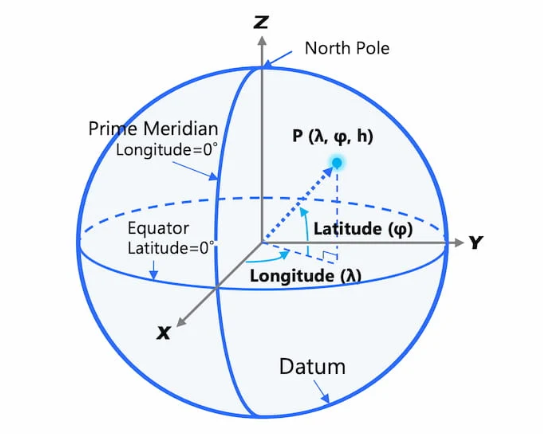
\includegraphics[width=0.5\linewidth]{figures/wgs84.png}
    \caption{Coordenadas GPS.}
    \label{fig:wgs84}
\end{figure}

\begin{figure}
     \centering
     \begin{subfigure}[b]{0.3\textwidth}
         \centering
         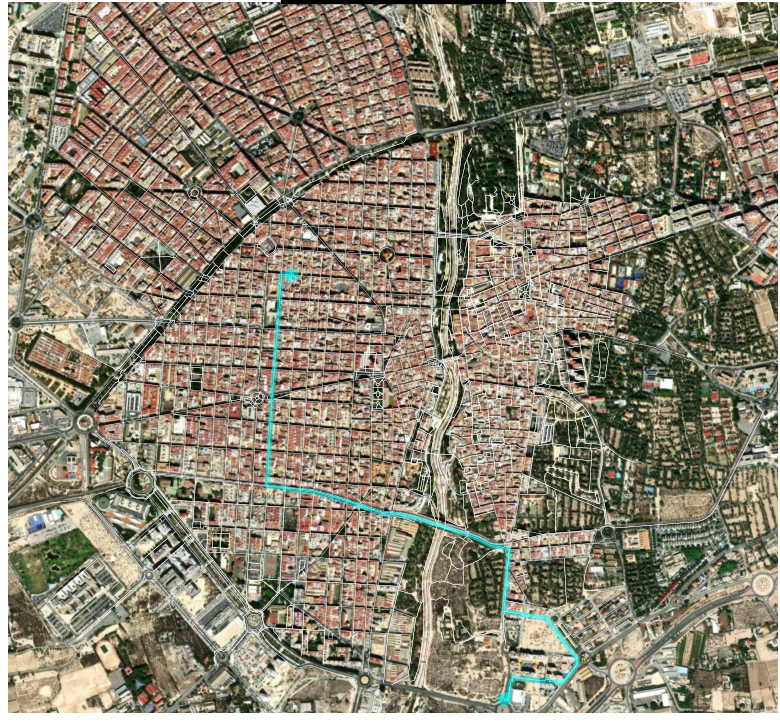
\includegraphics[width=\textwidth]{figures/map0.png}
         \caption{\texttt{map0.osm}}
         \label{fig:map0}
     \end{subfigure}
     \hfill
     \begin{subfigure}[b]{0.3\textwidth}
         \centering
         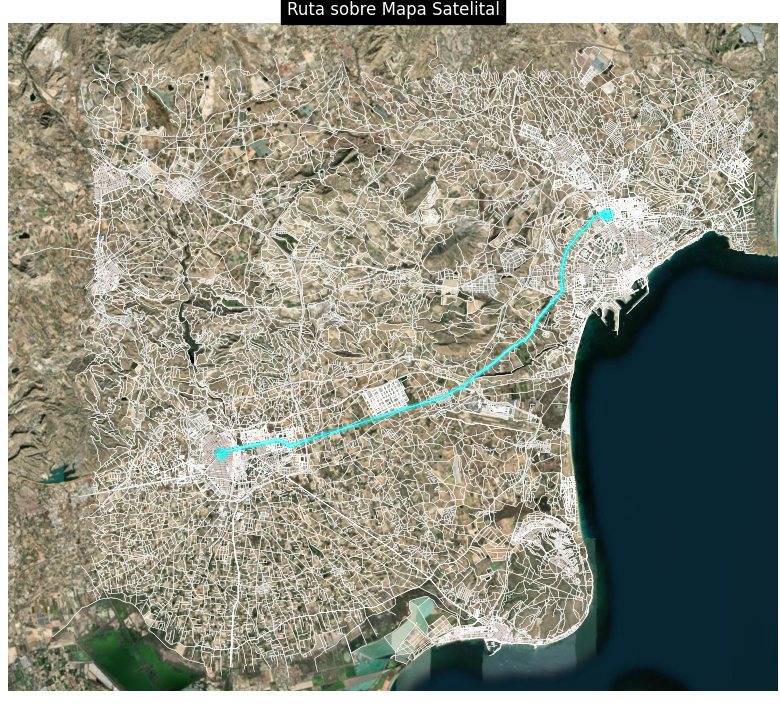
\includegraphics[width=\textwidth]{figures/map1.png}
         \caption{\texttt{map1.osm}}
         \label{fig:map1}
     \end{subfigure}
     \hfill
     \begin{subfigure}[b]{0.3\textwidth}
         \centering
         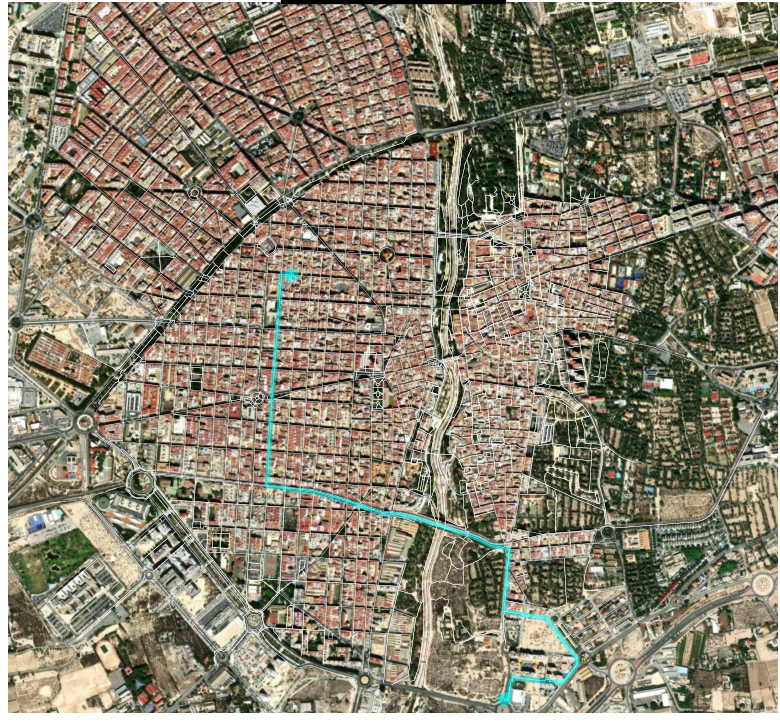
\includegraphics[width=\textwidth]{figures/map0.png}
         \caption{\texttt{map1.osm}}
         \label{fig:map2}
     \end{subfigure}
        \caption{Tres mapas de OSM.}
        \label{fig:tres_mapas}
\end{figure}

%\subsection{Carga del mapa como un grafo}


\subsection{Adaptación del algoritmo}
El algoritmo $A^*$ que se programó utilizaba cadenas de caracteres para nombrar los nodos. Además, cada nodo representaba una ciudad de España. En el caso que estudiaremos ahora, los nodos del mapa de OpenStreetMaps son posiciones GPS de calles y carreteras. Una calle está representada por diferentes nodos. Además, OpenStreetMaps mantiene una relación de conectividad entre nodos (id est, un grafo).

Usaremos la librería \texttt{osmnx} para cargar los datos de un mapa de OSM. Esto es fácil de hacer. Con esta línea cargaremos un mapa de nodos desde un fichero de OSM.
\begin{verbatim}
    G = ox.graph_from_xml("maps/map0.osm")
\end{verbatim}
Ahora nuestro grafo es \texttt{G}. Así pues, nuestro algoritmo usará este grafo \texttt{G}. El grafo \texttt{G} mantiene una lista de los nodos que están conectados: por ejemplo, calles que se cortan. Le pasaremos el grafo \texttt{G} al algoritmo para que lo use, igual que antes usábamos el grafo de ciudades:
\begin{verbatim}
    algoritmo = A_star_Algorithm_OSM(G)
\end{verbatim}
Igual que antes,  el grafo \texttt{G} se guardará en el algoritmo como \texttt{self.graph}. Con esto, para que nuestro algoritmo funcione, solamente hace falta adaptar las consultas que se hacían sobre el grafo anterior. En concreto, ahora hay que hacer las consultas sobre el grafo de tipo \texttt{osmnx}. Se anotan, a continuación, las funciones de la librería \texttt{osmnx} que necesitaremos: 
\begin{itemize}
    \item \textbf{Para saber si un nodo está en el mapa}. Ejemplo:
    \begin{verbatim}
        if start_name not in self.graph or destination_name not in self.graph:
            return None, None, None    
    \end{verbatim}
    \item Si deseamos \textbf{obtener los vecinos del nodo actual}. El siguiente código devuelve los nodos que están conectados con el nodo actual:
        \begin{verbatim}
            self.graph.neighbors(nodo_actual)
        \end{verbatim}
    \item \textbf{Distancia entre dos nodos conectados} del grafo:
        \begin{verbatim}
            datos_aristas = self.graph.get_edge_data(current_node_name, neighbor)
            rel_distance = datos_aristas[0].get('length')
        \end{verbatim}
    
    \item \textbf{Distancia \textit{flying distance} entre dos nodos (en metros)}. Se cebe implementar usando estas funciones:
        \begin{verbatim}
            lat, lon = self.graph.nodes[node_name]['y'], 
                self.graph.nodes[node_name]['x']
         ... 
            distance_meters = ox.distance.great_circle(lat1, lon1, lat2, lon2)
        \end{verbatim}    
\end{itemize}

\begin{exercise}
Complete las funciones del algoritmo proporcionado para que se pueda trabajar con grafos de tipo \texttt{osmnx}.\\
\textbf{EJERCICIO}\\
Modifique las funciones \texttt{self.get\_distance} y \texttt{self.compute\_flying\_distance} y \texttt{self.get\_neighbors}. Estas son funciones de la clase \texttt{A\_star\_Algorithm} que se han dejado vacías. A su vez, estas funciones deben llamar a las funciones de \texttt{osmnx} del grafo \texttt{self.graph} (que ahora es de tipo \texttt{osmnx}). Utilice el mapa \texttt{maps/map0.osm}, pues es más rápido cargarlo y hacer pruebas sobre él.    
\end{exercise}

\begin{exercise}
Pruebas a realizar: se anotan algunas coordenadas para trabajar con cada uno de los mapas:
\begin{itemize}
    \item \texttt{map0.osm} (Elche).
    \begin{verbatim}
        gps_origen = (38.266320, -0.706661)
        gps_destino = (38.166320, -0.686661)   
    \end{verbatim}
    
    \item \texttt{map1.osm} (Elche-Alicante).
    \begin{verbatim}
        gps_origen = (38.2694, -0.706661)
        gps_destino = (38.37, -0.5)
    \end{verbatim}

    \item \texttt{map2.osm} (Elche-Valencia).
    \begin{verbatim}
        gps_origen = (38.2694, -0.706661)
        gps_destino = (39.48, -0.362)
    \end{verbatim}
\end{itemize}
\end{exercise}

    
\subsection{Mejoras y tareas adicionales}
Nos damos cuenta de que la carga del mapa es lenta. Esto no resulta un gran inconveniente, pues en la aplicación que se está diseñando, esta acción se realiza una vez y, a continuación, el algoritmo puede calcular y servir muchas rutas. Nos da la sensación de que el algoritmo que se ha programado funciona con bastante rapidez, sin embargo, nos gustaría poder medir este tiempo. 

\begin{exercise}
Se desea medir el consumo del algoritmo en términos de tiempo de ejecución y memoria.\\
\textbf{EJERCICIO}\\
Cargue el mapa una vez y a continuación, genere 50 pares de coordenadas GPS de origen y destino aleatorias. Calcule el tiempo medio de ejecución. Intente normalizar el tiempo de ejecución respecto de la distancia de la ruta planificada por el algoritmo (rutas más largas requieren más tiempo, pues hay que explorar más nodos). El algoritmo se puede acelerar simplemente eliminando mucha de la información que se muestra por pantalla con \texttt{print()}. Busque, también, otras formas de acelerar el cálculo de las rutas.
\end{exercise}

\begin{exercise}
También resulta interesante que se plotee la posición GPS de todos los nodos que ha ido explorando el algoritmo. Recuerde que esta información se guarda en \texttt{self.visited\_nodes}. De esta manera el estudiante obtendrá una intuición de cómo funciona este algoritmo de búsqueda.
\end{exercise}

\end{document}
